\usepackage{pgf}
\usepackage{tikz}
\usetikzlibrary{arrows,automata}
\usepackage[latin1]{inputenc}
\usepackage{verbatim}


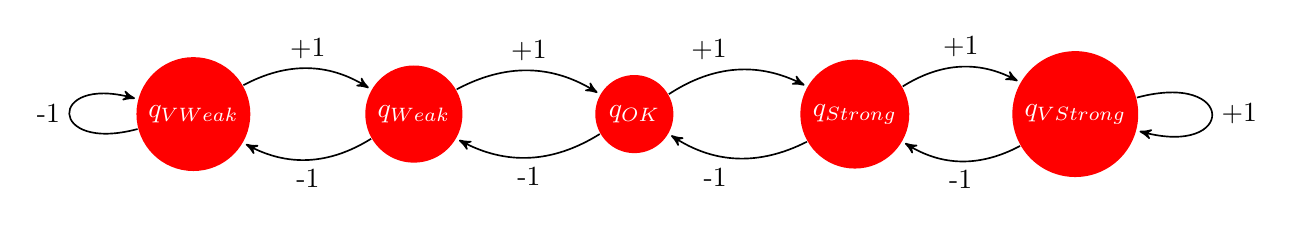
\begin{tikzpicture}[->,>=stealth',shorten >=1pt,auto,node distance=2.8cm,
                    semithick]
  \tikzstyle{every state}=[fill=red,draw=none,text=white]

  \node[state]         (A)                    {$q_{VWeak}$};
  \node[state]         (B) [right of=A]       {$q_{Weak}$};
  \node[state]         (C) [right of=B]       {$q_{OK}$};
  \node[state]         (D) [right of=C]       {$q_{Strong}$};
  \node[state]         (E) [right of=D]       {$q_{VStrong}$};

  \path (A) edge [bend left]  node {+1} (B)
                 edge [loop left]   node {-1}  (A) 
           (B) edge [bend left]  node {-1}  (A)
                 edge [bend left]  node {+1} (C)
           (C) edge [bend left]  node {-1}  (B)
                 edge [bend left]  node {+1} (D)
           (D) edge [bend left]  node {-1}  (C)
                 edge [bend left]  node {+1} (E)
           (E) edge [loop right] node {+1} (E)
                 edge [bend left]  node {-1}  (D);
\end{tikzpicture}
